\documentclass[11pt,compress,t,notes=noshow, xcolor=table]{beamer}
\usepackage[]{graphicx}\usepackage[]{color}
% maxwidth is the original width if it is less than linewidth
% otherwise use linewidth (to make sure the graphics do not exceed the margin)
\makeatletter
\def\maxwidth{ %
  \ifdim\Gin@nat@width>\linewidth
    \linewidth
  \else
    \Gin@nat@width
  \fi
}
\makeatother

\newcommand{\citebutton}[2]{%
\beamergotobutton{\href{#2}{#1}}%
}

\newcommand{\blu}[1]{\textcolor{blue}{#1}}
\newcommand{\org}[1]{\textcolor{orange}{#1}}
\newcommand{\ques}{\textbf{\textcolor{red}{Question:  }}}
\newcommand{\questionssofar}{\begin{frame}\frametitle{Any questions?}\end{frame}}

\newcommand\warning{%
 \makebox[1.4em][c]{%
 \makebox[0pt][c]{\raisebox{.1em}{\scriptsize!}}%
 \makebox[0pt][c]{\color{red}\normalsize$\bigtriangleup$}}}%

\definecolor{fgcolor}{rgb}{0.345, 0.345, 0.345}
\newcommand{\hlnum}[1]{\textcolor[rgb]{0.686,0.059,0.569}{#1}}%
\newcommand{\hlstr}[1]{\textcolor[rgb]{0.192,0.494,0.8}{#1}}%
\newcommand{\hlcom}[1]{\textcolor[rgb]{0.678,0.584,0.686}{\textit{#1}}}%
\newcommand{\hlopt}[1]{\textcolor[rgb]{0,0,0}{#1}}%
\newcommand{\hlstd}[1]{\textcolor[rgb]{0.345,0.345,0.345}{#1}}%
\newcommand{\hlkwa}[1]{\textcolor[rgb]{0.161,0.373,0.58}{\textbf{#1}}}%
\newcommand{\hlkwb}[1]{\textcolor[rgb]{0.69,0.353,0.396}{#1}}%
\newcommand{\hlkwc}[1]{\textcolor[rgb]{0.333,0.667,0.333}{#1}}%
\newcommand{\hlkwd}[1]{\textcolor[rgb]{0.737,0.353,0.396}{\textbf{#1}}}%
\let\hlipl\hlkwb

\usepackage{framed}
\makeatletter
\newenvironment{kframe}{%
 \def\at@end@of@kframe{}%
 \ifinner\ifhmode%
  \def\at@end@of@kframe{\end{minipage}}%
  \begin{minipage}{\columnwidth}%
 \fi\fi%
 \def\FrameCommand##1{\hskip\@totalleftmargin \hskip-\fboxsep
 \colorbox{shadecolor}{##1}\hskip-\fboxsep
     % There is no \\@totalrightmargin, so:
     \hskip-\linewidth \hskip-\@totalleftmargin \hskip\columnwidth}%
 \MakeFramed {\advance\hsize-\width
   \@totalleftmargin\z@ \linewidth\hsize
   \@setminipage}}%
 {\par\unskip\endMakeFramed%
 \at@end@of@kframe}
\makeatother

\definecolor{shadecolor}{rgb}{.97, .97, .97}
\definecolor{messagecolor}{rgb}{0, 0, 0}
\definecolor{warningcolor}{rgb}{1, 0, 1}
\definecolor{errorcolor}{rgb}{1, 0, 0}
\newenvironment{knitrout}{}{} % an empty environment to be redefined in TeX

\usepackage{alltt}
\newcommand{\SweaveOpts}[1]{}  % do not interfere with LaTeX
\newcommand{\SweaveInput}[1]{} % because they are not real TeX commands
\newcommand{\Sexpr}[1]{}       % will only be parsed by R
\newcommand{\xmark}{\ding{55}}%


\usepackage[english]{babel}
\usepackage[utf8]{inputenc}

\usepackage{dsfont}
\usepackage{verbatim}
\usepackage{amsmath}
\usepackage{amsfonts}
\usepackage{amssymb}
\usepackage{bm}
\usepackage{csquotes}
\usepackage{multirow}
\usepackage{longtable}
\usepackage{booktabs}
\usepackage{enumerate}
\usepackage[absolute,overlay]{textpos}
\usepackage{psfrag}
\usepackage{algorithm}
\usepackage{algpseudocode}
\usepackage{eqnarray}
\usepackage{arydshln}
\usepackage{tabularx}
\usepackage{placeins}
\usepackage{tikz}
\usepackage{setspace}
\usepackage{colortbl}
\usepackage{mathtools}
\usepackage{wrapfig}
\usepackage{bm}
\usepackage{amsmath}
\usepackage{pifont}

\usetikzlibrary{shapes.multipart,shapes,arrows,automata,positioning,calc,chains,trees, shadows}
\tikzset{
  %Define standard arrow tip
  >=stealth',
  %Define style for boxes
  punkt/.style={
    rectangle,
    rounded corners,
    draw=black, very thick,
    text width=6.5em,
    minimum height=2em,
    text centered},
  % Define arrow style
  pil/.style={
    ->,
    thick,
    shorten <=2pt,
    shorten >=2pt,}
}

\tikzstyle{vec}=[draw, rectangle, fill = white, minimum width=5mm, minimum height=1cm, inner sep = 2pt]

\usepackage{subfig}

% Defines macros and environments
\usepackage{../../style/lmu-lecture}


\let\code=\texttt
\let\proglang=\textsf

\setkeys{Gin}{width=0.9\textwidth}

\setbeamertemplate{frametitle}{\expandafter\uppercase\expandafter\insertframetitle}

\usepackage{bbm}
% basic latex stuff
\newcommand{\pkg}[1]{{\fontseries{b}\selectfont #1}} %fontstyle for R packages
\newcommand{\lz}{\vspace{0.5cm}} %vertical space
\newcommand{\dlz}{\vspace{1cm}} %double vertical space
\newcommand{\oneliner}[1] % Oneliner for important statements
{\begin{block}{}\begin{center}\begin{Large}#1\end{Large}\end{center}\end{block}}


%new environments
\newenvironment{vbframe}  %frame with breaks and verbatim
{
 \begin{frame}[containsverbatim,allowframebreaks]
}
{
\end{frame}
}

\newenvironment{vframe}  %frame with verbatim without breaks (to avoid numbering one slided frames)
{
 \begin{frame}[containsverbatim]
}
{
\end{frame}
}

\newenvironment{blocki}[1]   % itemize block
{
 \begin{block}{#1}\begin{itemize}
}
{
\end{itemize}\end{block}
}

\newenvironment{fragileframe}[2]{  %fragile frame with framebreaks
\begin{frame}[allowframebreaks, fragile, environment = fragileframe]
\frametitle{#1}
#2}
{\end{frame}}


\newcommand{\myframe}[2]{  %short for frame with framebreaks
\begin{frame}[allowframebreaks]
\frametitle{#1}
#2
\end{frame}}

\newcommand{\remark}[1]{
  \textbf{Remark:} #1
}


\newenvironment{deleteframe}
{
\begingroup
\usebackgroundtemplate{
\includegraphics[width=\paperwidth,height=\paperheight]{../style/color/red.png}}
 \begin{frame}
}
{
\end{frame}
\endgroup
}
\newenvironment{simplifyframe}
{
\begingroup
\usebackgroundtemplate{
\includegraphics[width=\paperwidth,height=\paperheight]{../style/color/yellow.png}}
 \begin{frame}
}
{
\end{frame}
\endgroup
}\newenvironment{draftframe}
{
\begingroup
\usebackgroundtemplate{
\includegraphics[width=\paperwidth,height=\paperheight]{../style/color/green.jpg}}
 \begin{frame}
}
{
\end{frame}
\endgroup
}
% https://tex.stackexchange.com/a/261480: textcolor that works in mathmode
\makeatletter
\renewcommand*{\@textcolor}[3]{%
  \protect\leavevmode
  \begingroup
    \color#1{#2}#3%
  \endgroup
}
\makeatother





\input{../../latex-math/basic-math.tex}
\input{../../latex-math/basic-ml.tex}


\def\rmA{{\mathbf{A}}}
\def\rmE{{\mathbf{E}}}
\def\rmR{{\mathbf{R}}}
\def\rmU{{\mathbf{U}}}
\def\rmW{{\mathbf{W}}}

\newcommand{\titlefigure}{figure/transformer_sq.png}
\newcommand{\learninggoals}{
\item Understand the limitations for long sequences
\item Understand the Segment Recurrence mechanism
\item Understand relative positional encodings}

\title{Transformer}
% \author{Bernd Bischl, Christoph Molnar, Daniel Schalk, Fabian Scheipl}
\institute{\href{https://slds-lmu.github.io/lecture_dl4nlp/}{slds-lmu.github.io/lecture\_dl4nlp}}
\date{}

\begin{document}
\lecturechapter{Transformer-XL}
\lecture{Deep Learning for NLP}

% ------------------------------------------------------------------------------

\begin{vbframe}{Limitation of the Transformer}

\vfill

\begin{figure}
\centering
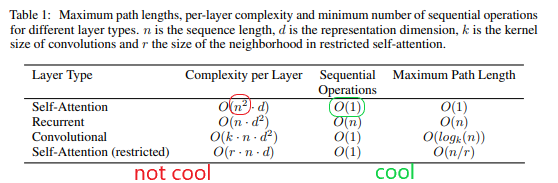
\includegraphics[width = 6.5cm]{figure/n_squared.png}\\ 
\footnotesize{Source:} \href{https://arxiv.org/pdf/1706.03762.pdf}{\footnotesize Vaswani et al. (2017)}
\end{figure}

\textbf{Advantage:}

\begin{itemize}
	\item Every token can \textit{directly} attend to each other token
	\item Cf. RNN: At worst $n$ sequential operations (last to first token)
\end{itemize}

\textbf{Severe Limitation:}

\begin{itemize}
	\item Every token attends to each other token (incl. itself)\\
				$\to$ We need to calculate $n^2$ attention weights
	\item Computational complexity of Transformer scales quadratically with the sequence length\\
				$\to$ Longer sequences are disproportionally expensive
\end{itemize}

\vfill

\end{vbframe}

% ------------------------------------------------------------------------------

\begin{vbframe}{Transformer-XL}

\vfill

\textbf{Key facts:}

\begin{itemize}
	\item Objective: Autoregressive Language Modeling task
	\item Transformer decoder model
	\item Addresses long sequences
	\item Assumption: \textit{No} infinite memory \& compute; limited resources
	\item (Possible) Solution Vanilla Transformer:
		\begin{itemize}
			\item Split corpus into shorter segments
			\item Limited contextual information
		\end{itemize}
	\item Solution Transformer-XL:
		\begin{itemize}
			\item Segment-level recurrence mechanism
			\item Able to model longer-term dependencies
		\end{itemize}
\end{itemize}

\vfill

\end{vbframe}

% ------------------------------------------------------------------------------

\begin{vbframe}{Transformer-XL}

\begin{figure}
\centering
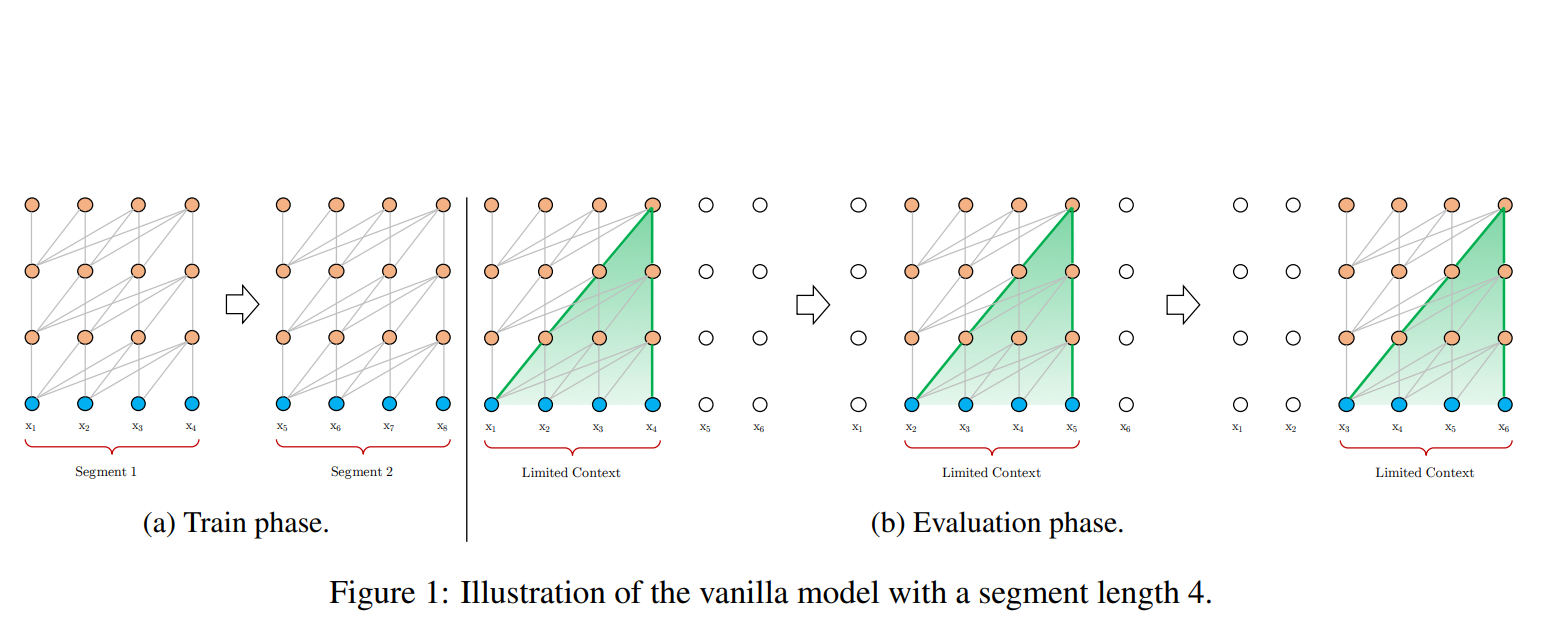
\includegraphics[width = 11.5cm]{figure/vanilla-trafo-seq4.png}\\ 
\footnotesize{Source:} \href{https://aclanthology.org/P19-1285.pdf}{\footnotesize Dai et al. (2019)}
\end{figure}

\begin{itemize}
		\item Contextual information limited to segments
		\item Does not respect semantic or syntactic boundaries
\end{itemize}

\end{vbframe}

% ------------------------------------------------------------------------------

\begin{vbframe}{Transformer-XL}

\begin{figure}
\centering
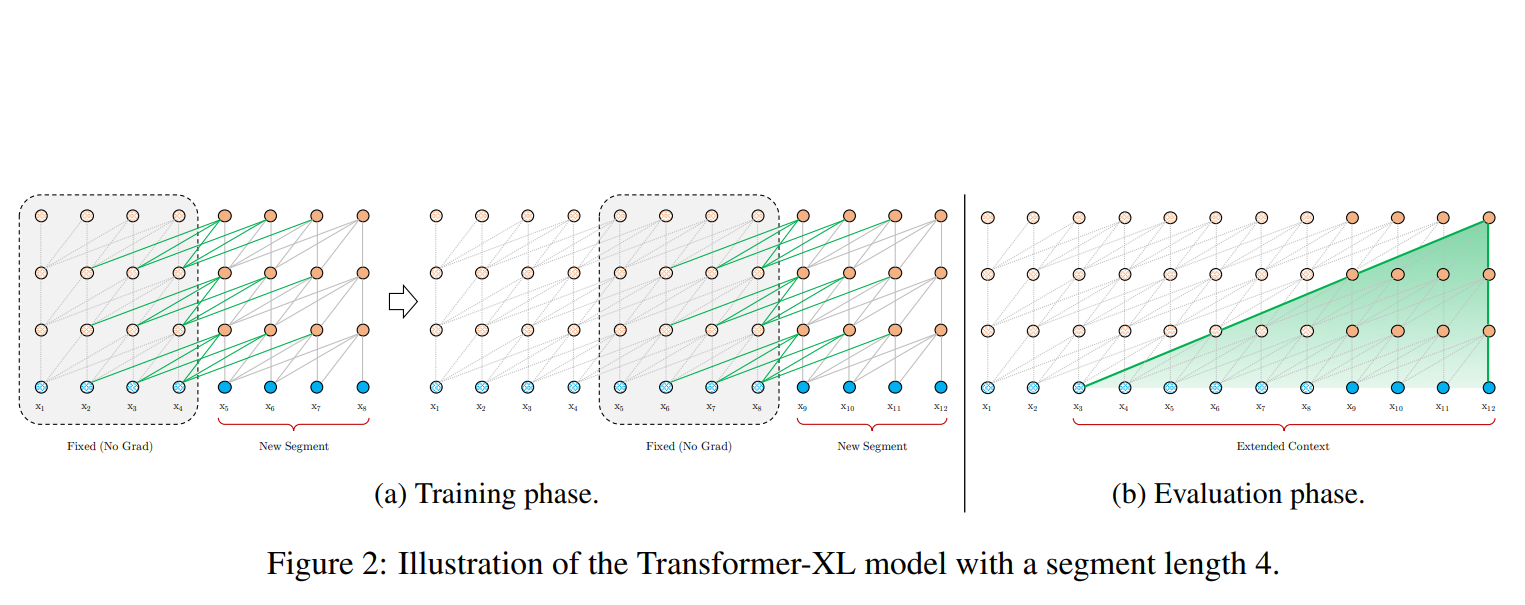
\includegraphics[width = 11.5cm]{figure/trafo-xl-seq4.png}\\ 
\footnotesize{Source:} \href{https://aclanthology.org/P19-1285.pdf}{\footnotesize Dai et al. (2019)}
\end{figure}

\begin{itemize}
		\item Caches hidden states from the previous segment
		\item Contextual information flows across segments
\end{itemize}

\end{vbframe}

% ------------------------------------------------------------------------------

\begin{vbframe}{Segment recurrence}

\begin{itemize}
		\item Let $s_\tau = [x_{\tau,1}, \hdots, x_{\tau,L}]$ and $s_{\tau+1} = [x_{\tau+1,1}, \hdots, x_{\tau+1,L}]$ be two consecutive segments of length $L$.
		\item Let $h_\tau^n \in \mathds{R}^{L\times d}$ denote the $n$-th layer hidden states for $s_\tau$.
		\item Using segment recurrence, the $n$-th layer hidden states for the following segment $s_{\tau+1}$ are computed as follows:
\end{itemize}

$$\tilde{h}_{\tau+1}^{n-1} = Concat[SG(h_{\tau}^{n-1}), h_{\tau+1}^{n-1}]$$

$$q_{\tau+1}^{n} = h_{\tau+1}^{n-1}W^\text{T}_q; \quad k_{\tau+1}^{n} = \tilde{h}_{\tau+1}^{n-1}W^\text{T}_k; \quad v_{\tau+1}^{n} = \tilde{h}_{\tau+1}^{n-1}W^\text{T}_v$$

$$h_{\tau+1}^{n} = Trafo(q_{\tau+1}^{n}, k_{\tau+1}^{n}, v_{\tau+1}^{n}),$$

\begin{itemize}
		\item[] where $SG(\cdot)$ stands for "`stop-gradient"'.
\end{itemize}

\end{vbframe}

% ------------------------------------------------------------------------------

\begin{vbframe}{Relative positional encodings}

\vfill

\textbf{Problem:}

\begin{itemize}
	\item \textit{Absolute} positional encodings (PE) would assign the same embedding to words in similar positions in both segments
	\item No positional difference between $x_{\tau,j}$ and $x_{\tau+1,j}$
\end{itemize}

\textbf{Solution:}

\begin{itemize}
	\item Inject information about the relative distance between a query vector and the respective key vectors directly into the Attention mechanism
	\item \textit{Comment:} Using relative PEs utterly necessary here, but also applicable independently of the segment recurrence
\end{itemize}

\begin{align*}
	\rmA_{i,j}^\text{abs} 
	&= \underbrace{ \rmE_{x_i}^\top \rmW_q^\top \rmW_k \rmE_{x_j} }_{(a)}
	+ \underbrace{\rmE_{x_i}^\top \rmW_q^\top \rmW_k \rmU_{j}}_{(b)} \\
	&+ \underbrace{\rmU_{i}^\top \rmW_q^\top \rmW_k \rmE_{x_j}}_{(c)}
	+ \underbrace{\rmU_{i}^\top \rmW_q^\top \rmW_k \rmU_{j}}_{(d)}. \vspace{-0.5em}
\end{align*}

\begin{align*}
	\rmA_{i,j}^\text{rel}
	&= \underbrace{ \rmE_{x_i}^\top \rmW_q^\top \rmW_{k,E} \rmE_{x_j} }_{(a)}
	+ \underbrace{\rmE_{x_i}^\top \rmW_q^\top \rmW_{k,R} \rmR_{i-j} }_{(b)} \\
	&+ \underbrace{u^\top \rmW_{k,E} \rmE_{x_j}}_{(c)}
	+ \underbrace{v^\top \rmW_{k,R} \rmR_{i-j}}_{(d)}.
\end{align*}

\end{vbframe}

% ------------------------------------------------------------------------------

\begin{vbframe}{Relative positional encodings}

\vfill

\textbf{Solution:}

\begin{itemize}
	\item Replace all absolute PEs with relative ones (fixed $+$ sinusoidal)\\
				$\to$ $\rmR_{i-j}$ instead of $\rmU_{j}$ in (b) and (d)
	\item Replace all positional query vectors with single trainable embeddings\\
				$\to$ $u$ and $v$ instead of $\rmU_{i}^\top \rmW_q^\top$ in (c) and (d)
	\item Use separate weight matrices for linearly projecting $\rmE$\\
				$\to$ $\rmW_{k,E}$ and $\rmW_{k,R}$ instead of $\rmW_{k}$
\end{itemize}

\vfill

\end{vbframe}

% ------------------------------------------------------------------------------

\endlecture
\end{document}
